\documentclass[12t,letterpaper]{article}

\newenvironment{proof}{\noindent{\bf Proof:}}{\qed\bigskip}

\newtheorem{theorem}{Theorem}
\newtheorem{corollary}{Corollary}
\newtheorem{lemma}{Lemma} 
\newtheorem{claim}{Claim}
\newtheorem{fact}{Fact}
\newtheorem{definition}{Definition}
\newtheorem{assumption}{Assumption}
\newtheorem{observation}{Observation}
\newtheorem{example}{Example}
\newcommand{\qed}{\rule{7pt}{7pt}}

\newcommand{\assignment}[4]{
\thispagestyle{plain} 
\newpage
\setcounter{page}{1}
\noindent
\begin{center}
\framebox{ \vbox{ \hbox to 6.28in
{\bf EE 122: Communication Networks \hfill #1}
\vspace{4mm}
\hbox to 6.28in
{\hspace{2.5in}\large\mbox{#2}}
\vspace{4mm}
\hbox to 6.28in
{{\it Handed Out: #3 \hfill Due: #4}}
}}
\end{center}
}

\newcommand{\solution}[3]{
\thispagestyle{plain} 
\newpage
\setcounter{page}{1}
\noindent
\begin{center}
\framebox{ \vbox{ \hbox to 6.28in
{\bf EE 122 \hfill #3}
\vspace{4mm}
\hbox to 6.28in
{\hspace{2.5in}\large\mbox{#2}}
\vspace{4mm}
\hbox to 6.28in
{#1 \hfill}
}}
\end{center}
\markright{#1}
}

\newenvironment{algorithm}
{\begin{center}
\begin{tabular}{|l|}
\hline
\begin{minipage}{1in}
\begin{tabbing}
\quad\=\qquad\=\qquad\=\qquad\=\qquad\=\qquad\=\qquad\=\kill}
{\end{tabbing}
\end{minipage} \\
\hline
\end{tabular}
\end{center}}

\def\Comment#1{\textsf{\textsl{$\langle\!\langle$#1\/$\rangle\!\rangle$}}}


\usepackage{amsmath, dsfont, tikz, float}
\usepackage{graphicx}

\usetikzlibrary{arrows,automata,positioning}

\oddsidemargin 0in
\evensidemargin 0in
\textwidth 6.5in
\topmargin -0.5in
\textheight 9.0in

\newenvironment{amatrix}[1]{%
  \left(\begin{array}{@{}*{#1}{c}|c@{}}
}{%
  \end{array}\right)
}

\makeatletter
\renewcommand*\env@matrix[1][*\c@MaxMatrixCols c]{%
  \hskip -\arraycolsep
  \let\@ifnextchar\new@ifnextchar
  \array{#1}}
\makeatother

\newcommand{\norm}[1]{\left\lVert #1 \right\rVert}
\newcommand{\?}{\stackrel{?}{=}}
\newcommand\given[1][]{\:#1\vert\:}


\begin{document}

\solution{Nikhil Unni}{HW1}{Spring 2016}
\pagestyle{myheadings}

\begin{enumerate}
  \item 
    \begin{enumerate}
      \item The plot is a straight line with y-intercept $0$, and with slope $\frac{3}{200}$. This continues until W*, or $(2000,30)$, at which point the line flattens off so that $\frac{dy}{dx} = 0$. This is because we've reached the link capacity of the bottleneck.
        Throughput is given by : $\frac{W(\text{\# of bits in a packet})}{RTT}$. And the RTT is the transmission time in addition to the propagation delay when sending to the sattelite. So we have:
        $$RTT = \frac{1}{1000} + 4(\frac{5*10^7}{3*10^8}) \approx \frac{2}{3}s$$
        So then throughput is given by : $\frac{W(10000)}{2/3} = \frac{3W}{200} \text{ Mbps}$
        So then, with some algebra:
        $$\frac{3W*}{200} = 30$$
        $$W* = 2000$$
        The average packet delay is : $\frac{1}{1000} + 2(\frac{5*10^7}{3*10^8}) = 0.334s$

      \item 
        The throughputs of A and B should be $15$ Mbps each, just from symmetry. So then the $RTT = \frac{2000(10000)}{15000000} = 1.33$ s, and time spent in the (now filled) queue should be $1.33 - \frac{1}{1000} - 4(\frac{5*10^7}{3*10^8}) = 0.666$ s. So then we know that the average packet delay now has to be : $\frac{1}{1000} + 0.666 + 2(\frac{5*10^7}{3*10^8}) \approx 1$ s.

      \item
        In the first case, we can use symmetry again to know that the two will have a $15$ Mbps throughput. And the delay would be $\frac{1.33}{2} = 0.665$. In the second case, we know what proportion of the available $30$ goes to each, so $A$ would get $20$ Mbps, and $B$ would get $10$ Mbps.
        
    \end{enumerate}
  \item For these problems, I took \textbf{first order approximations} of the answers in order to get a clean answer for part (v).
    \begin{enumerate}
      \item [(i)] Each RTT, we increase the window size by $1$. And this happens from $\frac{W}{2}$ to $W$, so in total, there are $W - \frac{W}{2} + 1 = \frac{W}{2} + 1 \approx \frac{W}{2}$ RTT between two loss events.
      \item [(ii)] Each RTT, we transmit $\frac{W}{2} + i$ packets. In total, between two loss events, this is given by:
        $$\sum_{i=W/2}^{W} i = \frac{3}{8}W(W+2) \approx \frac{3}{8}W^2$$
      \item [(iii)] For every loss event, we lose 1 packet. So then the packet loss rate must be:
        $$\frac{1}{3/8 W^2} = \frac{8}{3W^2}$$
      \item [(iv)] The throughput between loss events is the same as the overall throughput, since the distance between loss events is uniform. We already know the number of packets between two loss events is $\frac{3}{8}W^2$, and say the number of bits in the packet is $M$, so the number of bits between two loss events is $\frac{3}{8}MW^2$. And we know that the number of RTTs between two loss events is $\frac{W}{2}$, so the total time inbetween loss events must be $\frac{TW}{2}$. That means the throughput, which is the ratio of the two should be:
        $$=\frac{\frac{3}{8}MW^2}{\frac{TW}{2}} = \frac{3MW}{4T}$$
      \item [(v)] Call $q = \frac{8}{3W^2}$ the packet loss rate. Then, rearranging, we get $W = \sqrt{\frac{8}{3q}}$. So looking at our previous throughput equation, we have:
        $$\frac{3MW}{4T}$$
        $$=\frac{3M\sqrt{\frac{8}{3q}}}{4T}$$
        $$=\frac{3M\sqrt{8/3}}{4T \sqrt{q}}$$
        Call $K = \frac{3M \sqrt{8/3}}{4}$, then we get:
        $$=\frac{K}{T \sqrt{q}}$$
    \end{enumerate}

  \item 
    \begin{enumerate}
      \item 
        \includegraphics[width=1\textwidth]{im1}
      \item Using the preceding graph, we can see that the vector is slowly approaching the line $x_1=x_2$, meaning that after backing off, both have values of $\approx 54.54$, and build up until they both have $60$, then back off to $\approx 54.54$ again, forever. (Technically, the limit of the vector doesn't exist, since it will be ranging from $54$ to $60$ periodically.)
    \end{enumerate}

  \item 
    \begin{enumerate}
      \item 
        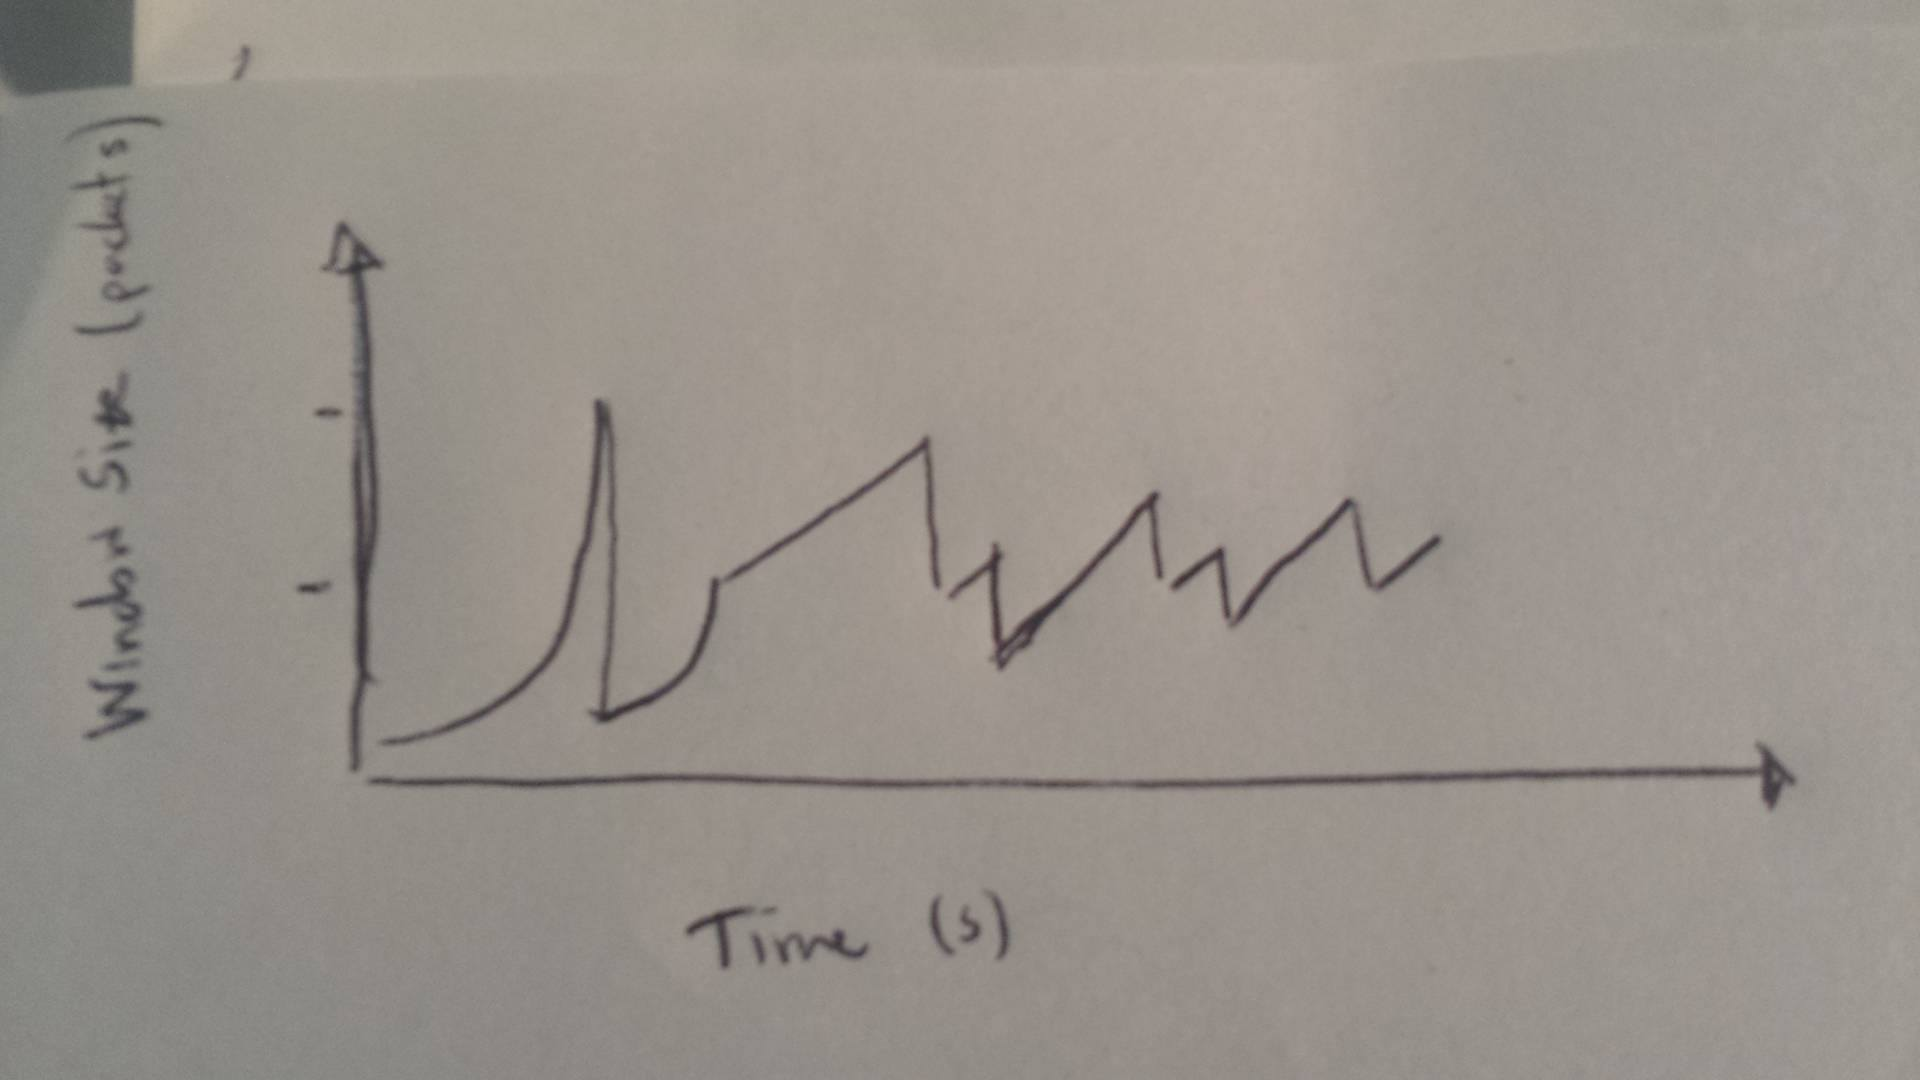
\includegraphics[width=1\textwidth]{im2}
      \item
        For a large $N$, the time spent will be dominated by the congestion control phase. Remember that the time spent inbetween packet losses is linear in the window size. Since the time inbetween packet losses is a linear increase, and the number of ``inbetween packet loss'' triangles is linear in the number of packets we need to send. So treat the slow start phase, and any irregularities in the tail end as a constant $b$. So then the total time spent to send a large $N$ packets is approximately $a + bN$, for some $a,b \in \mathds{R}$.
      \item The key factor that determines $b$ is the number of other computers attached the LAN. The more computers on the same Ethernet line, the more our two computers will have to wait, because of the randomized back-off schedule.
      \item The factors that will generally slow down the delivery of packets are overall network congestion as well as the link bottleneck of the entire network, which upperbounds the throughput of the connections.
    \end{enumerate}
    
  \item 
    \begin{enumerate}
      \item If $b > a$, then our constraint graph is just a right triangle with points at $(0,0), (0,a), (a,0)$. And at both points, the value of $x_1+x_2 = a$. However, if $b < a$, now we have a point at $(b,0)$, but $b < a$, so it cannot possibly be the maximum, and the maximum remains $a$. So the answer is $(a,0)$ in both cases.
      \item Intuitively, we know that any value other than $\frac{a}{2}$ for both will result in the minimum of the two being lower than $\frac{a}{2}$. So, from a simple argument of symmetry, if $b > \frac{a}{2}$, $x = (\frac{a}{2}, \frac{a}{2})$. Otherwise, if $b < \frac{a}{2}$, then clearly the max value we can get for the minimum is $b$, meaning $x = (b, a-b)$.
      \item If $b > a$, then we again have symmetry. So:
        $$log(x_1^2) = z \implies x_1 = \log(\frac{z}{2})$$
        $$2\log(\frac{z}{2}) = a \implies z = 2*10^{a/2}$$
        And so finally, the max $x$ value is : $(2*10^{a/2}, 2*10^{a/2})$.        
    \end{enumerate}
\end{enumerate}

\end{document}
